% Diapositivas Arquitecturas Analíticas - UdeSA

\documentclass{beamer}
\usetheme{metropolis}

\usepackage[spanish]{babel}
\usepackage[utf8]{inputenc}
\usepackage{graphicx}
\usepackage{tikz}
\usepackage{xcolor}
\usepackage{amsmath}

\usetikzlibrary{positioning,shapes.multipart,calc,arrows,shapes.geometric}

% Colores y configuración del template
\definecolor{primary}{RGB}{46, 204, 113}
\definecolor{secondary}{RGB}{52, 152, 219}
\definecolor{accent}{RGB}{231, 76, 60}
\definecolor{background}{RGB}{236, 240, 241}
\setbeamercolor{normal text}{fg=black,bg=background}
\setbeamercolor{structure}{fg=primary}
\setbeamercolor{alerted text}{fg=accent}

% Título
\title{Arquitecturas Analíticas}
\author{Gestión y Arquitectura de Datos}
\date{}

\begin{document}

% Portada
\begin{frame}
    \titlepage
    \begin{tikzpicture}[remember picture,overlay]
        \node[anchor=south west,inner sep=30pt] at (current page.south west) {
            
\includegraphics[height=1cm]{../misc/UdeSA.png}
        };
    \end{tikzpicture}
\end{frame}

% Introducción
\begin{frame}{Introducción}
    \begin{itemize}
        \item Permiten almacenar, procesar y analizar grandes volúmenes de datos
        \item Enfocadas en obtener conocimiento de datos históricos
        \item Integran datos de múltiples fuentes
        \item Requieren transformación y acceso eficiente para el análisis
        \item No hay una única solución, depende de la organización
    \end{itemize}
\end{frame}

% Conceptos Fundamentales - Data Warehouse
\begin{frame}{Data Warehouse}
    Un Data Warehouse es un lugar centralizado donde guardás datos ya procesados y estructurados para hacer análisis.
    
    \vspace{0.3cm}
    
    El proceso usa herramientas ETL (Extract, Transform, Load): extraés los datos, los transformás para limpiarlos y normalizarlos, y los cargás en el warehouse.
    
    \vspace{0.3cm}
    
    ``Schema-on-write'': los datos tienen que cumplir con un esquema predefinido antes de guardarlos. Esto garantiza consistencia y calidad, pero perdés flexibilidad.
\end{frame}

\begin{frame}{Data Warehouse: características}
    \begin{itemize}
        \item Pensados para consultas analíticas complejas sobre datos históricos
        \item Optimizados para múltiples usuarios haciendo consultas pesadas simultáneamente
        \item Arquitectura diseñada para lectura intensiva, no para escribir constantemente
        \item Datos estructurados y normalizados, más fáciles de consultar y analizar
    \end{itemize}
\end{frame}

\begin{frame}{Data Warehouse}
    \begin{center}
        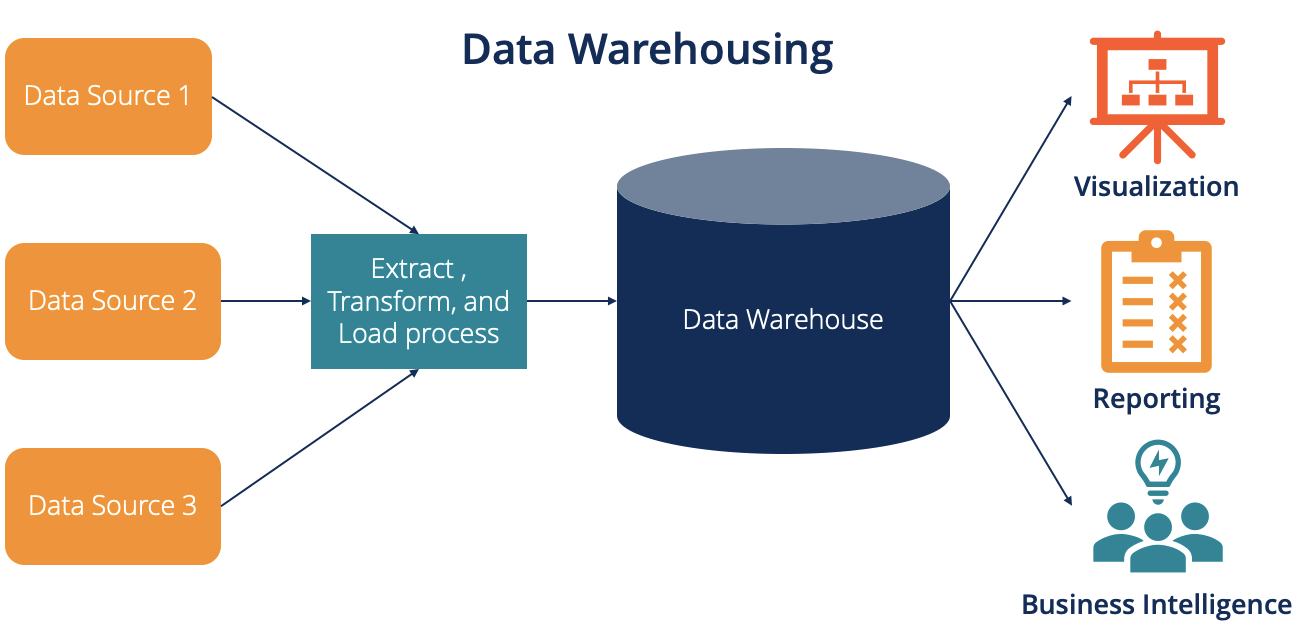
\includegraphics[width=0.9\textwidth]{img/datawarehouse.png}
    \end{center}
\end{frame}

\begin{frame}{Data Warehouse: ventajas y desventajas}
    \begin{columns}
        \begin{column}{0.5\textwidth}
            \textbf{Ventajas:}
            \begin{itemize}
                \item Fuente única de verdad
                \item Datos validados y estructurados
                \item Los analistas pueden enfocarse en análisis en vez de limpiar datos
            \end{itemize}
        \end{column}
        \begin{column}{0.5\textwidth}
            \textbf{Desventajas:}
            \begin{itemize}
                \item Construcción y mantenimiento costosos
                \item Puede llevar bastante tiempo
                \item Menos flexibilidad, especialmente con muchas fuentes diferentes
            \end{itemize}
        \end{column}
    \end{columns}
\end{frame}

% Conceptos Fundamentales - Data Lake
\begin{frame}{Data Lake}
    En un \textbf{Data Lake} guardás los datos en crudo, sin procesarlos mucho y sin que tengan que cumplir con un esquema específico cuando los cargás.
    
    \vspace{0.3cm}
    
    \textit{Schema-on-read}: no definís el esquema antes de guardar, sino cuando leés los datos. Útil para datos no estructurados o semi-estructurados (logs, imágenes, videos, sensores).
    
    \vspace{0.3cm}
    
    La idea es capturar y guardar todo lo que puedas, incluso si todavía no sabés si va a ser útil. Como el almacenamiento es relativamente barato, no es tan costoso guardar datos que quizás no uses.
    
    \vspace{0.3cm}
    
    \alert{\textbf{Riesgo}}: sin gobernanza, puede convertirse en un ``data swamp''.
\end{frame}

\begin{frame}{Data Lake}
    \begin{center}
        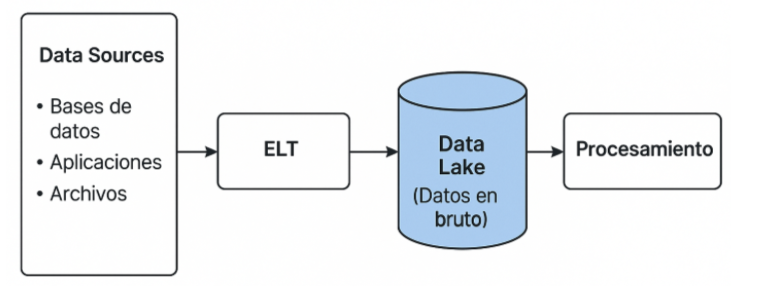
\includegraphics[width=0.9\textwidth]{img/arq_data_lake.png}
    \end{center}
\end{frame}

\begin{frame}{Data Lake: ventajas y desventajas}
    \begin{columns}
        \begin{column}{0.5\textwidth}
            \textbf{Ventajas:}
            \begin{itemize}
                \item Flexibilidad para datos diversos
                \item Almacenamiento relativamente barato
                \item Útil para investigación y ML
                \item Permite guardar datos sin saber su uso futuro
            \end{itemize}
        \end{column}
        \begin{column}{0.5\textwidth}
            \textbf{Desventajas:}
            \begin{itemize}
                \item Sin gobernanza puede ser difícil de usar
                \item Sin catalogación y metadata, difícil encontrar lo que guardaste
                \item Consultas más lentas: hay que procesar el esquema cada vez
            \end{itemize}
        \end{column}
    \end{columns}
\end{frame}

% Conceptos Fundamentales - Data Mart
\begin{frame}{Data Mart}
    Un Data Mart es un subconjunto de un Data Warehouse o Data Lake enfocado en un área específica, como un departamento o caso de uso particular.
    
    \vspace{0.3cm}
    
    En vez de que los usuarios naveguen por todo el warehouse, les das acceso solo a los datos que realmente necesitan. Esto hace que sea más rápido de consultar y más fácil de entender.
    
    \vspace{0.3cm}
    
    Pueden construirse como subconjuntos de un warehouse centralizado (mantiene consistencia) o directamente desde las fuentes de datos.
\end{frame}

\begin{frame}{Data Mart}
    \begin{center}
        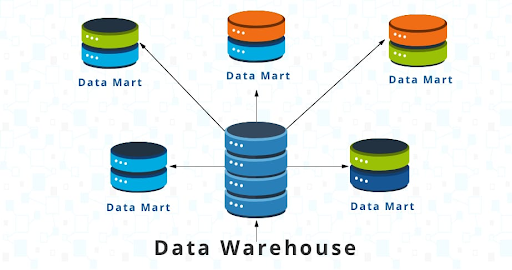
\includegraphics[width=0.9\textwidth]{img/datamart.png}
    \end{center}
\end{frame}

\begin{frame}{Data Mart: ventajas y desventajas}
    \begin{columns}
        \begin{column}{0.5\textwidth}
            \textbf{Ventajas:}
            \begin{itemize}
                \item Acceso rápido y enfocado
                \item Más fácil de entender
                \item Optimizado para casos de uso específicos
            \end{itemize}
        \end{column}
        \begin{column}{0.5\textwidth}
            \textbf{Desventajas:}
            \begin{itemize}
                \item Riesgo de inconsistencias
                \item Riesgo de diferentes versiones de los mismos datos
                \item Puede llevar a decisiones contradictorias
            \end{itemize}
        \end{column}
    \end{columns}
\end{frame}

% Arquitecturas Clásicas - Inmon
\begin{frame}{Arquitectura Inmon}
    En la arquitectura Inmon primero construís un Data Warehouse corporativo integrado y normalizado, y después derivás los Data Marts específicos para cada área o departamento.
    
    \vspace{0.3cm}
    
    \textbf{Enfoque bottom-up}: primero la base corporativa, luego los Data Marts específicos.
    
    \vspace{0.3cm}
    
    El warehouse está normalizado (típicamente en tercera forma normal), sin redundancia. Es la única fuente de verdad: todos los Data Marts comparten la misma base de datos subyacente.
\end{frame}

\begin{frame}{Arquitectura Inmon: características}
    Requiere bastante planificación y diseño inicial: identificar todas las fuentes de datos, entender cómo se relacionan, y diseñar un esquema normalizado. Tenes que saber muy bien lo que querés.
    
    \vspace{0.3cm}
    
    Los Data Marts son vistas o subconjuntos del warehouse corporativo. Cada uno está optimizado para las necesidades de un departamento específico, pero todos comparten la misma fuente de datos.
    
    \vspace{0.3cm}
    
    Esto puede llevar tiempo, pero el resultado es un sistema robusto y bien integrado.
\end{frame}

\begin{frame}{Arquitectura Inmon}
    \begin{center}
        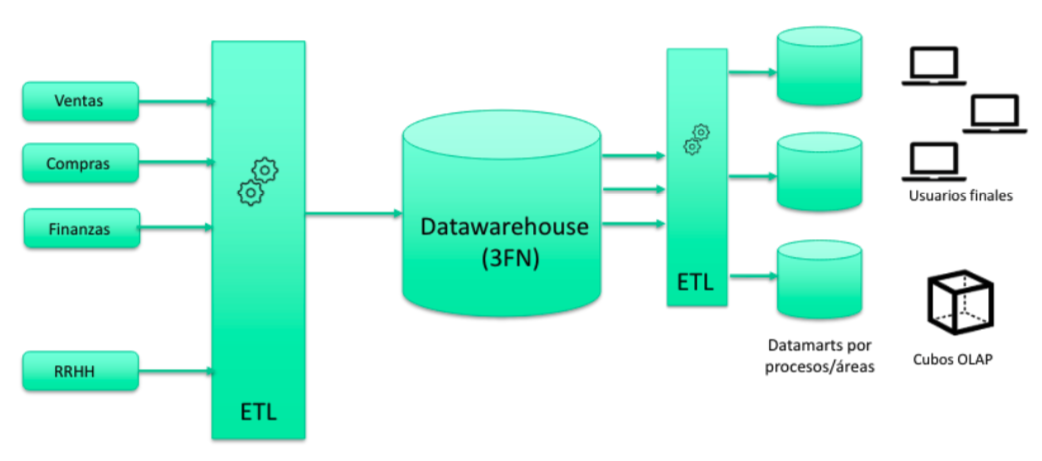
\includegraphics[width=0.9\textwidth]{img/inmon.png}
    \end{center}
\end{frame}

\begin{frame}{Arquitectura Inmon: ventajas y desventajas}
    \begin{columns}
        \begin{column}{0.5\textwidth}
            \textbf{Ventajas:}
            \begin{itemize}
                \item Visión integrada y consistente
                \item Elimina inconsistencias que aparecen cuando cada departamento construye su propio sistema
                \item Sistema robusto y bien integrado
                \item Todos los análisis se basan en la misma información centralizada
            \end{itemize}
        \end{column}
        \begin{column}{0.5\textwidth}
            \textbf{Desventajas:}
            \begin{itemize}
                \item Más lento de implementar inicialmente
                \item Hay que construir el warehouse antes de entregar valor
                \item Requiere identificar todas las fuentes desde el principio
                \item Puede llevar tiempo antes de ver resultados
            \end{itemize}
        \end{column}
    \end{columns}
\end{frame}

% Arquitecturas Clásicas - Kimball
\begin{frame}{Arquitectura Kimball}
    En la arquitectura Kimball empezás construyendo Data Marts específicos que resuelven problemas concretos, y después gradualmente los integrás.
    
    \vspace{0.3cm}
    
    \textbf{Enfoque top-down}: primero los Data Marts específicos, luego la integración gradual.
    
    \vspace{0.3cm}
    
    En vez de construir un Data Warehouse corporativo completo desde el principio, identificás un caso de uso con valor claro y construís un Data Mart dimensional. Cuando funciona, construís el siguiente, y así.
\end{frame}

\begin{frame}{Arquitectura Kimball: dimensiones conformadas}
    Las dimensiones conformadas permiten que los Data Marts se integren gradualmente sin perder consistencia.
    
    \vspace{0.3cm}
    
    Son dimensiones que se comparten entre múltiples Data Marts, con el mismo significado y estructura en todos ellos. Por ejemplo, una dimensión de tiempo o de producto que se usa de la misma forma en todos los Data Marts.
    
    \vspace{0.3cm}
    
    Esto garantiza consistencia y permite aprender y ajustar el enfoque basándote en los resultados antes de comprometerte con una arquitectura completa.
\end{frame}

\begin{frame}{Arquitectura Kimball}
    \begin{center}
        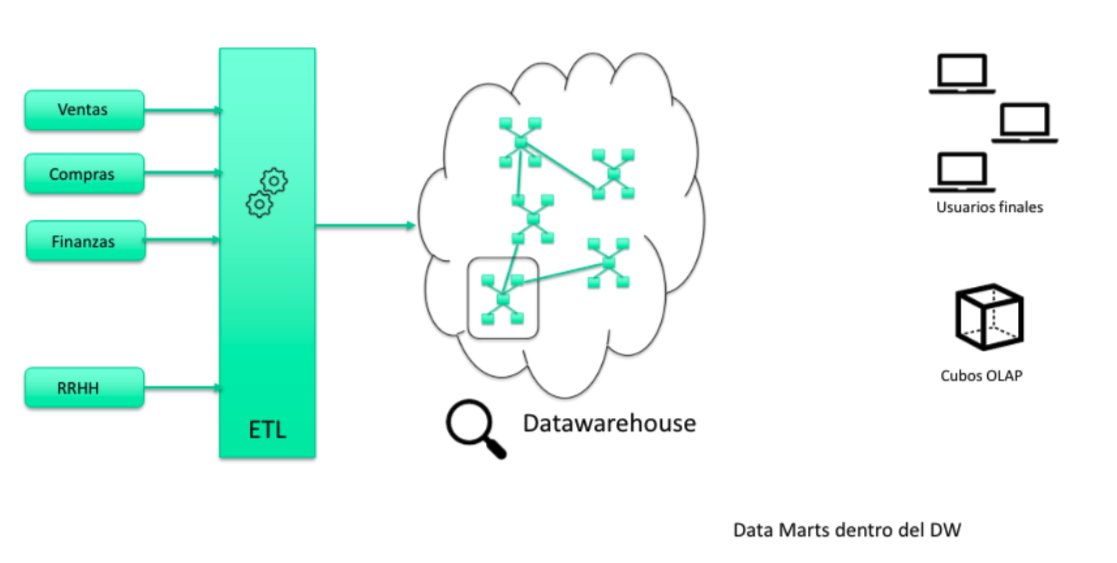
\includegraphics[width=0.9\textwidth]{img/kimball.png}
    \end{center}
\end{frame}

\begin{frame}{Arquitectura Kimball: ventajas y desventajas}
    \begin{columns}
        \begin{column}{0.5\textwidth}
            \textbf{Ventajas:}
            \begin{itemize}
                \item Podés entregar valor más rápido
                \item Al empezar con un Data Mart específico, tenés algo funcionando en mucho menos tiempo
                \item Permite aprender y ajustar el enfoque basándote en los resultados
            \end{itemize}
        \end{column}
        \begin{column}{0.5\textwidth}
            \textbf{Desventajas:}
            \begin{itemize}
                \item Necesitás  asegurarte de que los Data Marts se construyan de forma que puedan integrarse después
                \item Si no se planifican las dimensiones conformadas, la integración futura puede ser difícil
                \item Riesgo de inconsistencias similares a los que Inmon intenta evitar
            \end{itemize}
        \end{column}
    \end{columns}
\end{frame}

% Modelos Dimensionales - Introducción
\begin{frame}{Modelos Dimensionales}
    Los modelos dimensionales son una forma de organizar datos pensada específicamente para facilitar el análisis y la consulta.
    
    \vspace{0.3cm}
    
    La estructura básica tiene dos tipos principales de tablas: tablas de hechos y tablas de dimensión.
\end{frame}

\begin{frame}{Modelos Dimensionales: componentes}
    \begin{columns}
        \begin{column}{0.5\textwidth}
            \textbf{Tablas de Hechos}
            \begin{itemize}
                \item Tienen las métricas o medidas que querés analizar
                \item Ejemplos: ventas, ingresos, cantidad de productos vendidos
                \item Cualquier otra medida numérica relevante
            \end{itemize}
        \end{column}
        \begin{column}{0.5\textwidth}
            \textbf{Tablas de Dimensión}
            \begin{itemize}
                \item Dan el contexto para analizar esos hechos
                \item Describen quién, qué, cuándo, dónde y cómo ocurrieron los hechos
                \item Ejemplos: tiempo, producto, cliente, ubicación
            \end{itemize}
        \end{column}
    \end{columns}
\end{frame}

% Modelos Dimensionales - Estrella
\begin{frame}{Modelo Dimensional Estrella}
    El modelo dimensional estrella se llama así porque la estructura se parece a una estrella: una tabla de hechos en el centro y múltiples tablas de dimensión conectadas directamente a ella. Este modelo es el más simple y común.
\end{frame}

\begin{frame}{Modelo Estrella: estructura}
    La tabla de hechos tiene las medidas numéricas y claves foráneas que la conectan con cada tabla de dimensión.
    
    \vspace{0.3cm}
    
    Cada tabla de dimensión está completamente desnormalizada: toda la información relevante está guardada directamente en esa tabla. Por ejemplo, una dimensión de producto podría tener en una sola tabla: ID, nombre, categoría, marca, proveedor, precio, etc.
\end{frame}

\begin{frame}{Modelo Dimensional Estrella}
    \begin{center}
        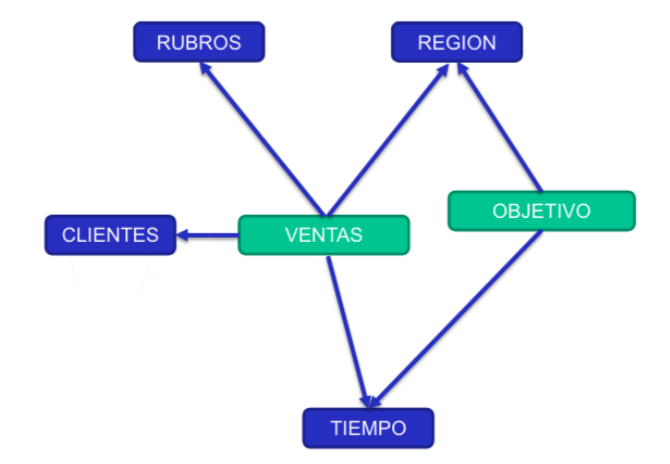
\includegraphics[width=0.9\textwidth]{img/star_schema.png}
    \end{center}
\end{frame}

\begin{frame}{Modelo Estrella: ventajas y desventajas}
    \begin{columns}
        \begin{column}{0.5\textwidth}
            \textbf{Ventajas:}
            \begin{itemize}
                \item Simplicidad: consultas típicas requieren solo un join
                \item Consultas más rápidas y fáciles de escribir
                \item Más intuitivo para usuarios finales
            \end{itemize}
        \end{column}
        \begin{column}{0.5\textwidth}
            \textbf{Desventajas:}
            \begin{itemize}
                \item La desnormalización puede llevar a redundancia de datos
                \item Información de las dimensiones se repite para cada registro relacionado
                \item Redundancia consume espacio, aunque beneficio en simplicidad y rendimiento vale la pena
            \end{itemize}
        \end{column}
    \end{columns}
\end{frame}

% Modelos Dimensionales - Snowflake
\begin{frame}{Modelo Dimensional Snowflake}
    El modelo dimensional snowflake es una variación del modelo estrella donde las tablas de dimensión están normalizadas, dividiéndose en múltiples tablas relacionadas.
    
    \vspace{0.3cm}
    
    La estructura se parece a un copo de nieve, con la tabla de hechos en el centro y las dimensiones extendiéndose en múltiples niveles.
\end{frame}

\begin{frame}{Modelo Snowflake: estructura}
    En vez de tener toda la información de una dimensión en una sola tabla desnormalizada, la información se divide en múltiples tablas relacionadas.
    
    \vspace{0.3cm}
    
    Por ejemplo, en vez de una dimensión de producto con categoría, marca y proveedor directamente, un modelo snowflake podría tener tablas separadas de producto, categoría, marca y proveedor, todas relacionadas entre sí.
    
    \vspace{0.3cm}
    
    Esto crea una estructura jerárquica que se extiende en múltiples niveles, como los brazos de un copo de nieve.
\end{frame}

\begin{frame}{Modelo Dimensional Snowflake}
    \begin{center}
        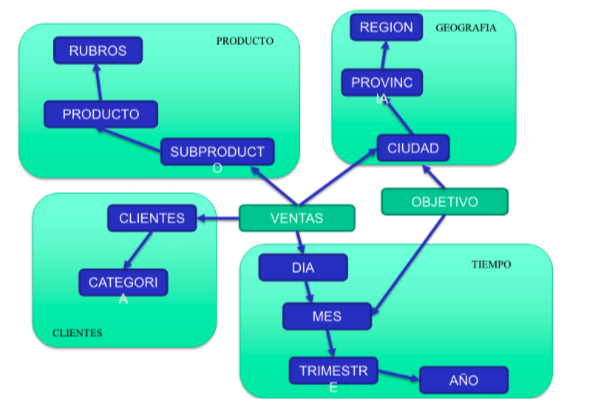
\includegraphics[width=0.9\textwidth]{img/snowflake_schema.png}
    \end{center}
\end{frame}

\begin{frame}{Modelo Snowflake: ventajas y desventajas}
    \begin{columns}
        \begin{column}{0.5\textwidth}
            \textbf{Ventajas:}
            \begin{itemize}
                \item La normalización reduce la redundancia de datos
                \item Mantenimiento más fácil cuando hay cambios en la estructura
                \item Menor consumo de espacio
            \end{itemize}
        \end{column}
        \begin{column}{0.5\textwidth}
            \textbf{Desventajas:}
            \begin{itemize}
                \item Las consultas se vuelven más complejas
                \item Requieren múltiples joins para reconstruir la información completa
                \item Consultas más lentas y difíciles de escribir y optimizar
                \item Menos intuitivo para usuarios finales
            \end{itemize}
        \end{column}
    \end{columns}
\end{frame}

% Cierre
\begin{frame}{Terminamos}
    \begin{center}
        \Large{\textbf{¿Dudas?\\¿Consultas?}}
    \end{center}
    \begin{tikzpicture}[remember picture,overlay]
        \node[anchor=south,inner sep=30pt] at (current page.south) {
            
\includegraphics[height=1cm]{../misc/UdeSA.png}
        };
    \end{tikzpicture}
\end{frame}

\end{document}

